%%%%%%%%%%%%%%%%%%%%%%%%%%%%%%%%%%%%%%%%%
% Beamer Presentation
% LaTeX Template
% Version 1.0 (10/11/12)
%
% This template has been downloaded from:
% http://www.LaTeXTemplates.com
%
% License:
% CC BY-NC-SA 3.0 (http://creativecommons.org/licenses/by-nc-sa/3.0/)
%
%%%%%%%%%%%%%%%%%%%%%%%%%%%%%%%%%%%%%%%%%

%----------------------------------------------------------------------------------------
%	PACKAGES AND THEMES
%----------------------------------------------------------------------------------------

\documentclass[UTF8,aspectratio=169,14pt]{ctexbeamer}

\usepackage{hyperref}
\hypersetup{
	colorlinks=true,
	linkcolor=red,
	anchorcolor=blue,
	citecolor=green
}

\mode<presentation> {
	
	% The Beamer class comes with a number of default slide themes
	% which change the colors and layouts of slides. Below this is a list
	% of all the themes, uncomment each in turn to see what they look like.
	
	%\usetheme{default}
	%\usetheme{AnnArbor}
	%\usetheme{Antibes}
	%\usetheme{Bergen}
	%\usetheme{Berkeley}
	%\usetheme{Berlin}
	%\usetheme{Boadilla}
	%\usetheme{CambridgeUS}
	%\usetheme{Copenhagen}
	%\usetheme{Darmstadt}
	%\usetheme{Dresden}
	%\usetheme{Frankfurt}
	%\usetheme{Goettingen}
	%\usetheme{Hannover}
	%\usetheme{Ilmenau}
	%\usetheme{JuanLesPins}
	%\usetheme{Luebeck}
	\usetheme{Madrid}
	%\usetheme{Malmoe}
	%\usetheme{Marburg}
	%\usetheme{Montpellier}
	%\usetheme{PaloAlto}
	%\usetheme{Pittsburgh}
	%\usetheme{Rochester}
	%\usetheme{Singapore}
	%\usetheme{Szeged}
	%\usetheme{Warsaw}
	
	% As well as themes, the Beamer class has a number of color themes
	% for any slide theme. Uncomment each of these in turn to see how it
	% changes the colors of your current slide theme.
	
	%\usecolortheme{albatross}
	%\usecolortheme{beaver}
	%\usecolortheme{beetle}
	%\usecolortheme{crane}
	%\usecolortheme{dolphin}
	%\usecolortheme{dove}
	%\usecolortheme{fly}
	%\usecolortheme{lily}
	%\usecolortheme{orchid}
	%\usecolortheme{rose}
	%\usecolortheme{seagull}
	%\usecolortheme{seahorse}
	%\usecolortheme{whale}
	%\usecolortheme{wolverine}
	
	%\setbeamertemplate{footline} % To remove the footer line in all slides uncomment this line
	%\setbeamertemplate{footline}[page number] % To replace the footer line in all slides with a simple slide count uncomment this line
	
	%\setbeamertemplate{navigation symbols}{} % To remove the navigation symbols from the bottom of all slides uncomment this line
}

\usepackage{graphicx} % Allows including images
\graphicspath{{./figs/}}
\usepackage{booktabs} % Allows the use of \toprule, \midrule and \bottomrule in tables
\usepackage{longtable}
\usepackage{listings}
\usepackage{xcolor}
\lstset{numbers=left, %设置行号位置
	numberstyle=\tiny, %设置行号大小
	keywordstyle=\color{blue}, %设置关键字颜色
	commentstyle=\color[cmyk]{1,0,1,0}, %设置注释颜色
	frame=single, %设置边框格式
	escapeinside=``, %逃逸字符(1左面的键),用于显示中文
	%breaklines, %自动折行
	extendedchars=false, %解决代码跨页时,章节标题,页眉等汉字不显示的问题
	xleftmargin=2em,xrightmargin=2em, aboveskip=1em, %设置边距
	tabsize=4, %设置tab空格数
	showspaces=false %不显示空格
}
% Fonts
% \usepackage{libertine}
% \setmonofont{Courier}
\setCJKsansfont[ItalicFont=Noto Serif CJK SC Black, BoldFont=Noto Sans CJK SC Black]{Noto Sans CJK SC}


%----------------------------------------------------------------------------------------
%	TITLE PAGE
%----------------------------------------------------------------------------------------

\title[第3讲]{第3讲 :Virtual Machine Monitor} % The short title appears at the bottom of every slide, the full title is only on the title page
\subtitle{第一节:Overview }
\author{陈渝} % Your name
\institute[清华大学] % Your institution as it will appear on the bottom of every slide, may be shorthand to save space
{
	清华大学计算机系 \\ % Your institution for the title page
	\medskip
	\textit{yuchen@tsinghua.edu.cn} % Your email address
}
\date{\today} % Date, can be changed to a custom date


\begin{document}

\begin{frame}
\titlepage % Print the title page as the first slide
\end{frame}

%\begin{frame}
%\frametitle{提纲} % Table of contents slide, comment this block out to remove it
%\tableofcontents % Throughout your presentation, if you choose to use \section{} and \subsection{} commands, these will automatically be printed on this slide as an overview of your presentation
%\end{frame}
%
%%----------------------------------------------------------------------------------------
%%	PRESENTATION SLIDES
%%----------------------------------------------------------------------------------------
%
%%------------------------------------------------
%\section{第一节:课程概述} % Sections can be created in order to organize your presentation into discrete blocks, all sections and subsections are automatically printed in the table of contents as an overview of the talk
%%------------------------------------------------
%-------------------------------------------------
\begin{frame}[plain]
	\frametitle{Introduction}
	
	
	
	\begin{columns}
		
		\begin{column}{.4\textwidth}
			
			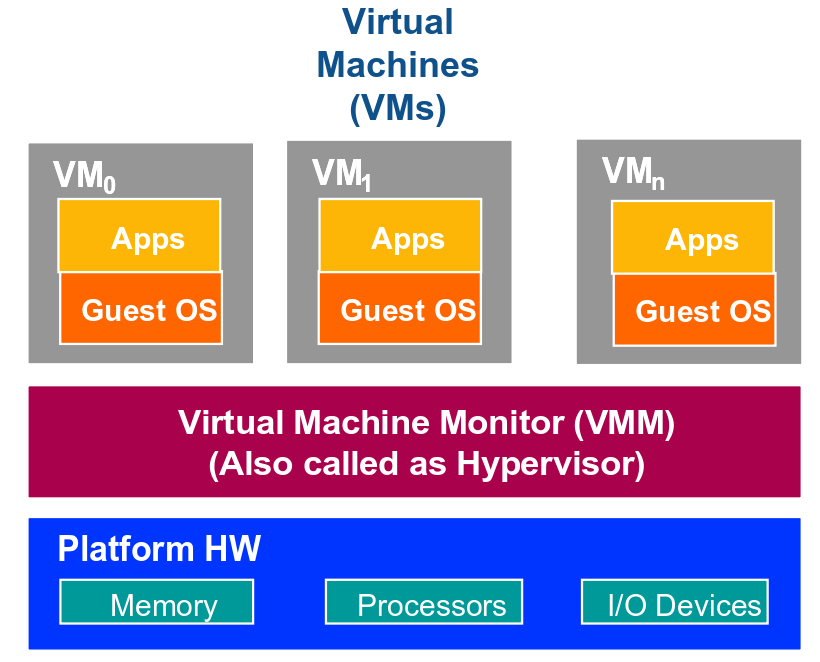
\includegraphics[width=1.\textwidth]{vmm-overview}
			
		\end{column}
		
		\begin{column}{.6\textwidth}
			
		
			\begin{block}{What is Virtualization}
				Virtualization is a term that refers to the abstraction of computer resources [wikipedia]
			\end{block}
		
			\begin{block}{Wisdom}
				All computer problems can be solved with another layer of redirection [Donald E. Knuth (高德纳), Stanford University]
			\end{block}

		\end{column}
		
		
	\end{columns}
	
	
\end{frame}

%-------------------------------------------------
\begin{frame}[plain]
	\frametitle{Introduction -- taxonomy}



	\begin{columns}

	\begin{column}{.3\textwidth}
	
	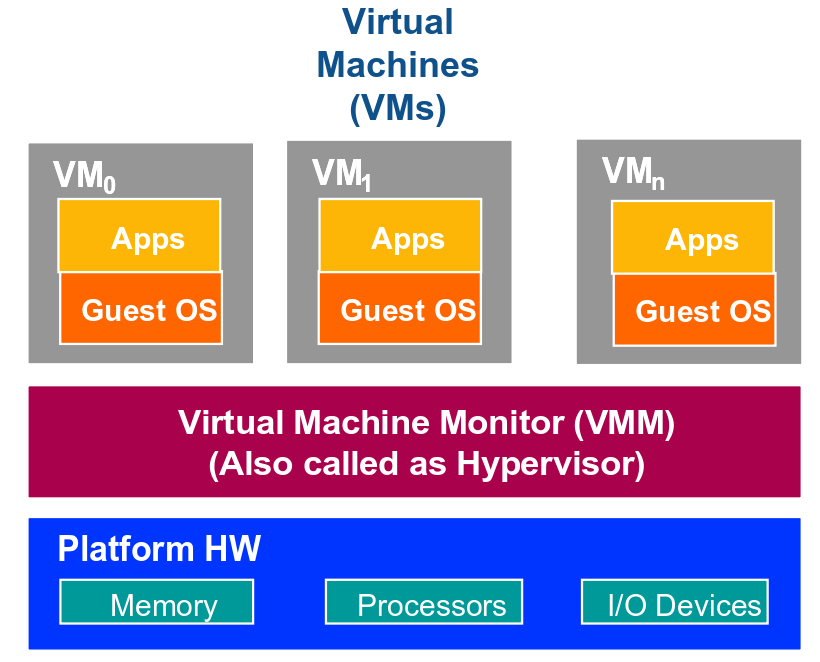
\includegraphics[width=1.\textwidth]{vmm-overview}
	
	\end{column}

	\begin{column}{.7\textwidth}
	
%	\Large
%    OS Structure	
%	\begin{itemize}
%	\item Simple kernel
%%	\item Monolithic kernel
%%	\item Micro kernel
%%	\item Exokernel
%%	\item VMM, etc...
%	\end{itemize}	

	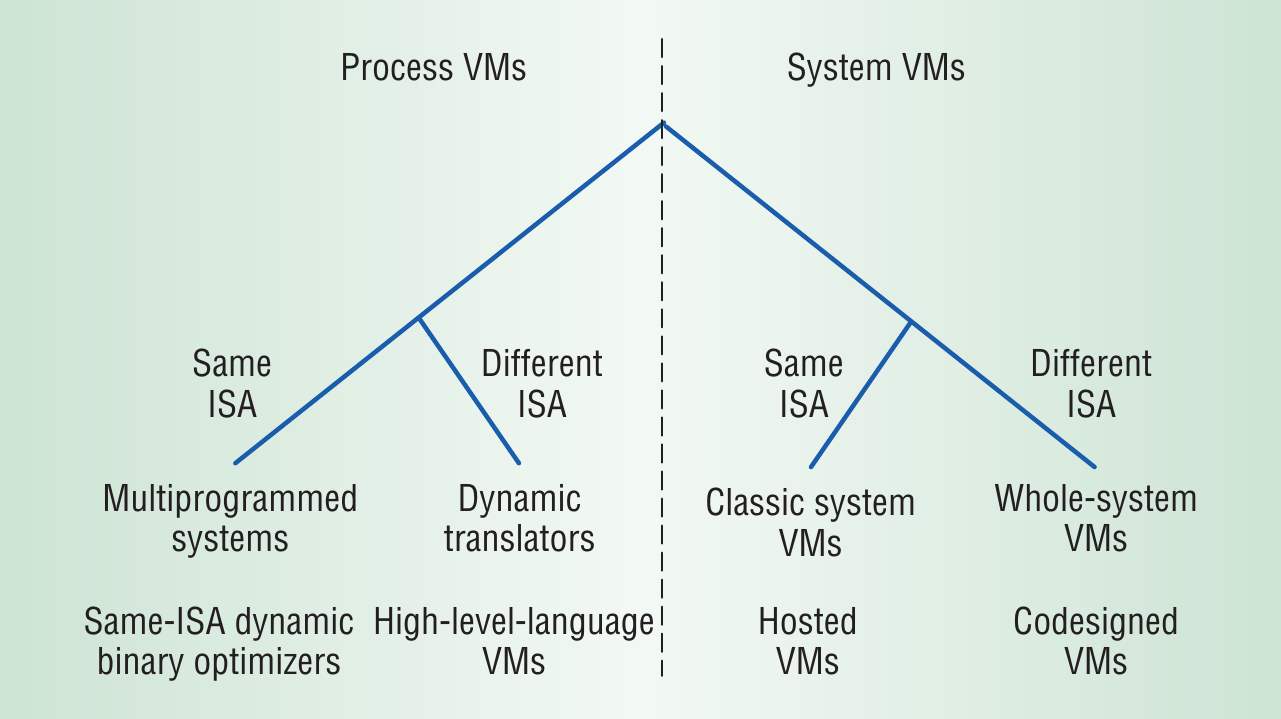
\includegraphics[width=1.\textwidth]{vm-taxonomy}
	
	\tiny	
	from James E.Smith,     IEEE computer Society2005	
	\end{column}
	
    
\end{columns}


\end{frame}

%-------------------------------------------------
\begin{frame}[plain]
	\frametitle{Introduction -- different layer of virtualization}
	
	
	
	\begin{columns}
		
		\begin{column}{.3\textwidth}
			
			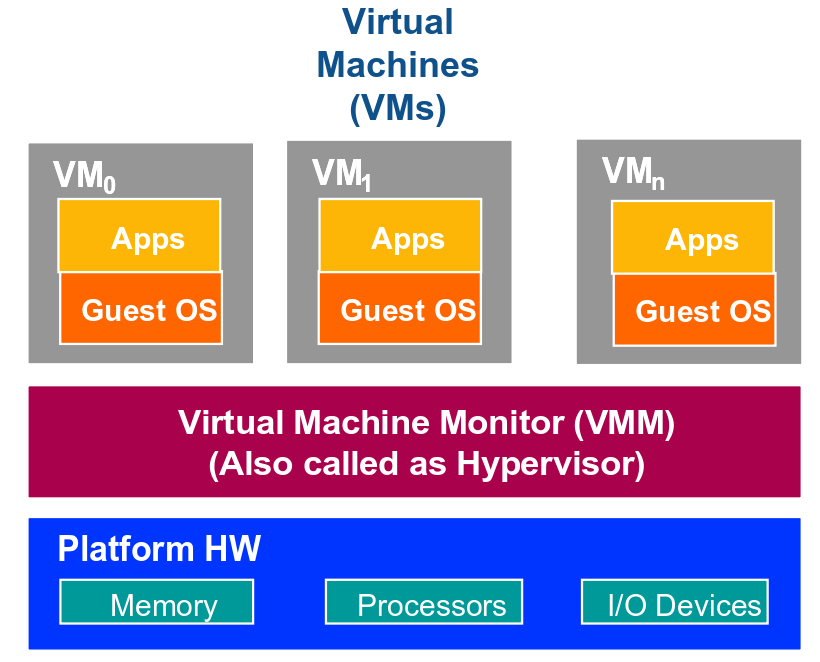
\includegraphics[width=1.\textwidth]{vmm-overview}
			
		\end{column}
		
		\begin{column}{.5\textwidth}
			
			%	\Large
			%    OS Structure	
			%	\begin{itemize}
			%	\item Simple kernel
			%%	\item Monolithic kernel
			%%	\item Micro kernel
			%%	\item Exokernel
			%%	\item VMM, etc...
			%	\end{itemize}	
			
			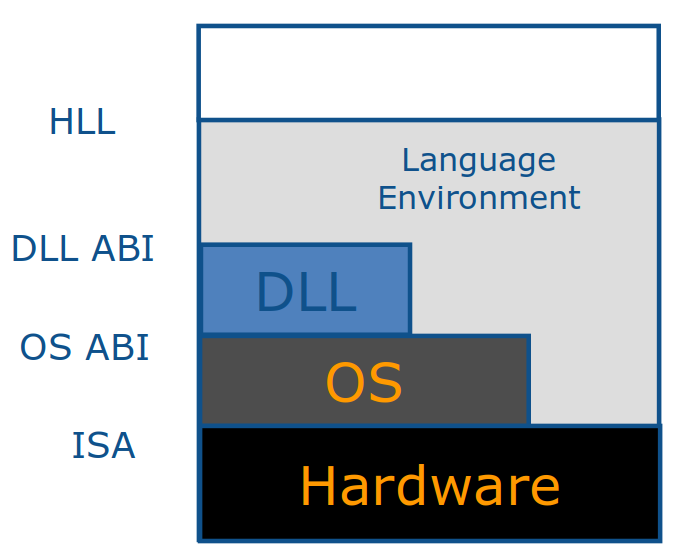
\includegraphics[width=1.\textwidth]{vm-layer}
			
			
		\end{column}
		
		
	\end{columns}
	
	
\end{frame}


%-------------------------------------------------
\begin{frame}[plain]
	\frametitle{Introduction -- VMM}
	
	
	
	\begin{columns}
		
		\begin{column}{.5\textwidth}
			
			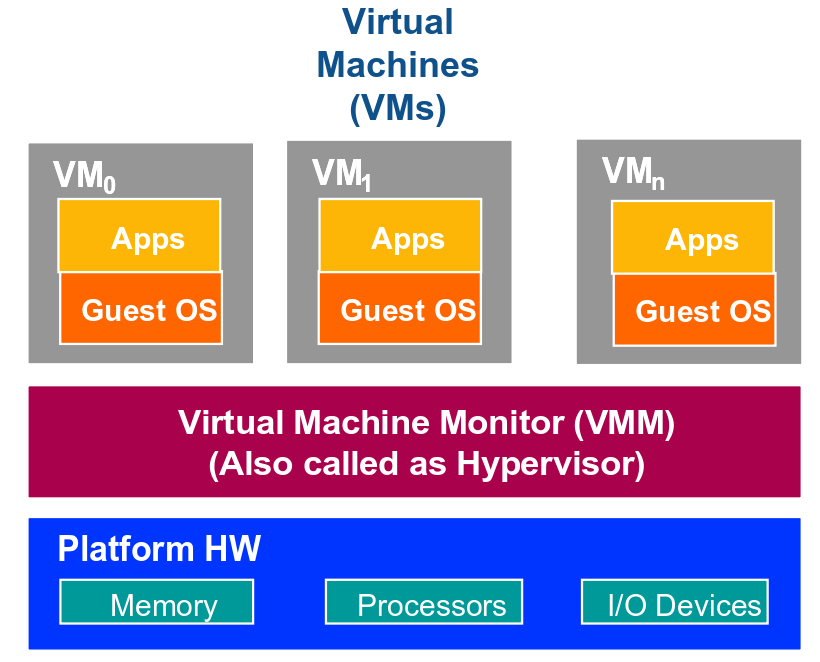
\includegraphics[width=1.\textwidth]{vmm-overview}
			
		\end{column}
		
		\begin{column}{.5\textwidth}
			
			\begin{block}{Virtual Machine Monitor, VMM}
	VMM transforms the single machine interface into the illusion of many. Each of these interfaces (virtual machines) is an efficient replica of the original computer system, complete with all of the processor instructions [Robert P. Goldberg, 1974]
			\end{block}
			
%			\begin{block}{Virtual Machine Monitor, VMM}
%				A virtual machine is implemented by adding software to an execution platform to give it the appearance of a different platform, or for that matter, to give the appearance of multiple platforms. [. E. Smith and Ravi Nair, “An Overview of Virtual Machine Architectures”.]
%			\end{block}
		\end{column}
		
		
	\end{columns}
	
	
\end{frame}

%-------------------------------------------------
\begin{frame}[plain]
	\frametitle{Introduction -- VMM}
	
	
	
	\begin{columns}
		
		\begin{column}{.5\textwidth}
			
			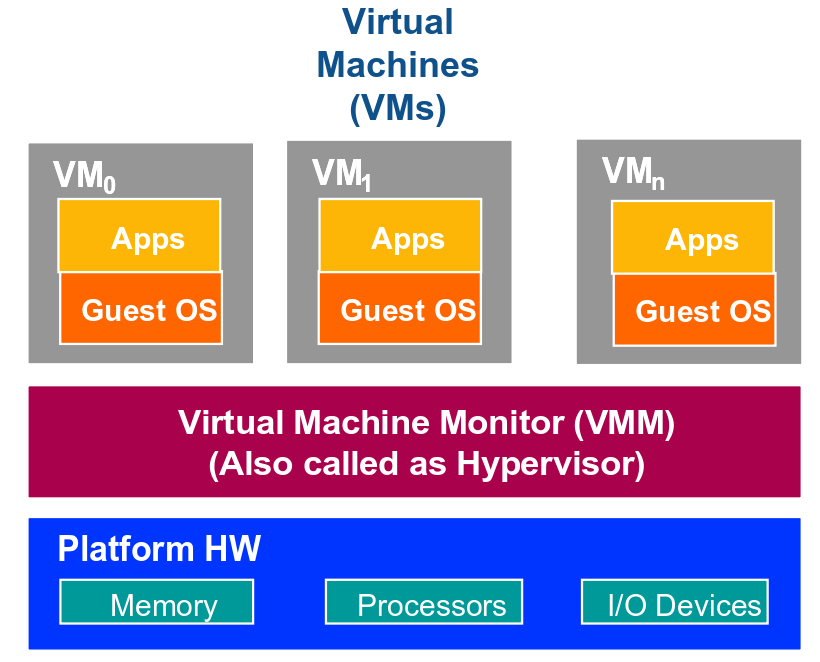
\includegraphics[width=1.\textwidth]{vmm-overview}
			
		\end{column}
		
		\begin{column}{.5\textwidth}
			
%			\begin{block}{Virtual Machine Monitor, VMM}
%				VMM transforms the single machine interface into the illusion of many. Each of these interfaces (virtual machines) is an efficient replica of the original computer system, complete with all of the processor instructions [Robert P. Goldberg, 1974]
%			\end{block}
			
			\begin{block}{Virtual Machine Monitor, VMM}
				A virtual machine is implemented by adding software to an execution platform to give it the appearance of a different platform, or for that matter, to give the appearance of multiple platforms. [J.E. Smith, “An Overview of Virtual Machine Architectures”]
			\end{block}
		\end{column}
		
		
	\end{columns}
	
	
\end{frame}


%-------------------------------------------------
\begin{frame}[plain]
	\frametitle{Introduction -- Why VMM?}
	
	
	
	\begin{columns}
		
		\begin{column}{.5\textwidth}
			
			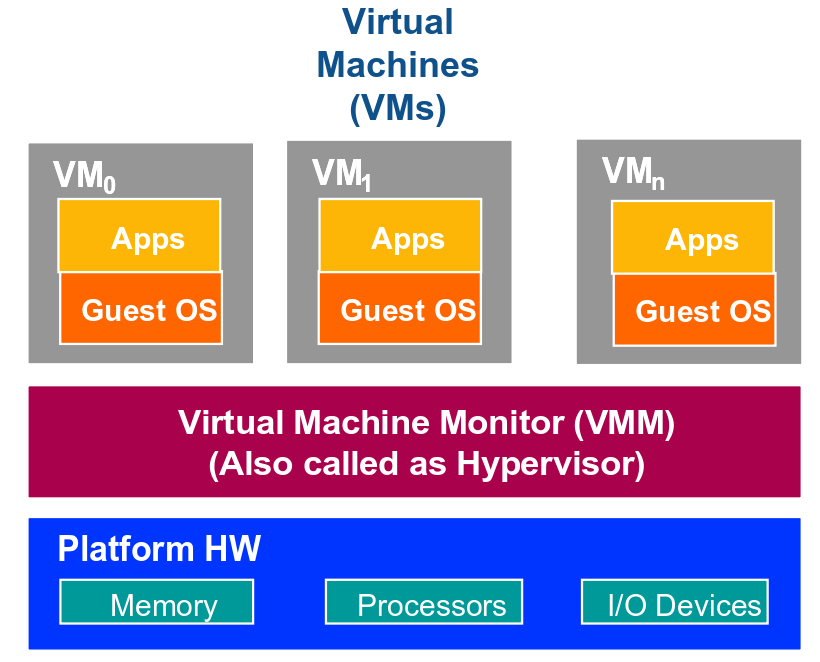
\includegraphics[width=1.\textwidth]{vmm-overview}
			
		\end{column}
		
		\begin{column}{.5\textwidth}
		
		Before there were data centers... 
		\begin{itemize}
			\item Many early commercial computers were mainframes
			\item powerful computation, highly reliable, extensive I/O capabilities
			\item for computing/data-intensive  apps 
			
		\end{itemize} 	
        IBM	System/360 hardware and CP/CMS system software: Virtualizable Architecture
		\end{column}
		
		
	\end{columns}
		
\end{frame}


%-------------------------------------------------
\begin{frame}[plain]
	\frametitle{Introduction -- Why VMM?}
	
	
	
	\begin{columns}
		
		\begin{column}{.5\textwidth}
			
			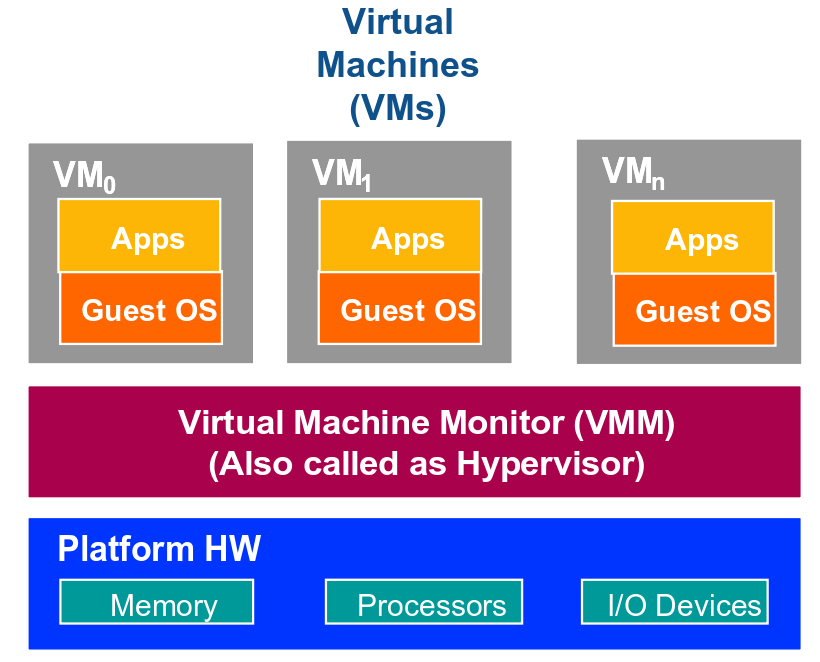
\includegraphics[width=1.\textwidth]{vmm-overview}
			
		\end{column}
		
		\begin{column}{.5\textwidth}
			
			Now there were data centers... 
			\begin{itemize}
				\item Many computers were servers connected in the world.
				\item powerful computation, highly reliable, extensive I/O capabilities
				\item for computing/data-intensive apps 

				
			\end{itemize} 	
			 x86/ARM and Linux/KVM, vmware, xen, etc. system software: Virtualizable Architecture
		\end{column}
		
		
	\end{columns}
	
\end{frame}


%-------------------------------------------------
\begin{frame}[plain]
	\frametitle{Introduction -- Essential characteristics of VMM}
	
	
	
	\begin{columns}
		
		\begin{column}{.5\textwidth}
			
			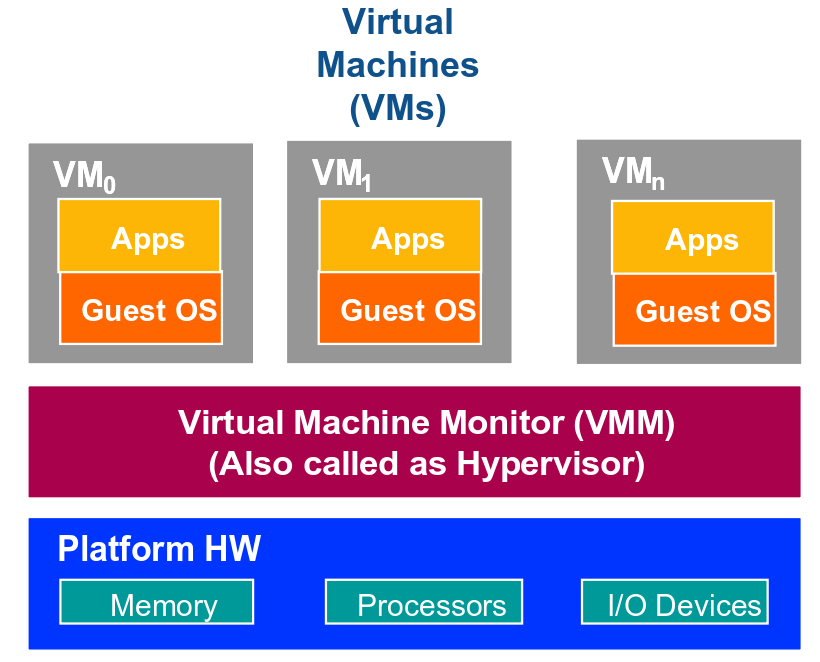
\includegraphics[width=1.\textwidth]{vmm-overview}
			
		\end{column}
		
		\begin{column}{.5\textwidth}
			
	     \begin{itemize}
			\item Equivalence: Essentially identical virtual platform, except
			\begin{itemize}
				\item Differences caused by the availability of system resources. e.g. memory size

			\end{itemize} \pause
			
			\item Isolation, or resource control 
			\begin{itemize}
				\item VMM is in complete control of system resources
				
			\end{itemize} \pause
			
			\item Efficiency
			\begin{itemize}
				\item At worst only minor decreases in speed
				\item speed $>>$ emulators, software interpreters (simulators)
				
			\end{itemize}
		
     	\end{itemize}	
	
		\end{column}
		
		
	\end{columns}
	
	
\end{frame}


%-------------------------------------------------


\end{document}